\documentclass[a4paper,12pt]{article}
\usepackage[utf8]{inputenc}
\usepackage{fancyhdr}
\usepackage{mathrsfs}
\usepackage{amsmath}
\usepackage{sidecap}
\usepackage{float}
\usepackage{bm}
\usepackage{blindtext}
\usepackage{gensymb}
\usepackage{amsfonts}
\usepackage{ragged2e}
\usepackage[a4paper,margin=25mm]{geometry}
\usepackage{authblk}
\usepackage{caption}
\usepackage{graphicx}
\usepackage[usenames,dvipsnames]{color,xcolor}
\usepackage{listings}
\usepackage{hyperref}
\usepackage{lastpage}
\usepackage{xepersian}

\settextfont{BNazanin}
\setlatintextfont{Liberation Serif}

% \setlength{\droptitle}{-10em}
%%%%%%%%%%%%%%%%%%%%%%%%%%%%%%%%%%%%%%%%%%%%%%%%5
\lstset{
language=C++,
frame=trBL,  
numbers=left,
numberstyle=\scriptsize,
frameround=fttt,
showspaces=false,           % Leerzeichen anzeigen ?
showtabs=false,             % Tabs anzeigen ?
xleftmargin=25pt,
xrightmargin=10pt,
framexleftmargin=17pt,
framexrightmargin=5pt,
framexbottommargin=4pt,
showstringspaces=false ,
breaklines=true,
texcl=true,
basicstyle=\setLTR\footnotesize\ttfamily,
  commentstyle= \itshape,
  keywordstyle=\bfseries,
  belowcaptionskip=12pt,
  aboveskip=15pt,
  belowskip=7pt
}  
%%%%%%%%%%%%%%%%%%%%%%%%%%%%%%%%%%%%%%%%%%%%%%%%%

\pagestyle{fancy}
\rhead{\small{آیزینگ}}
\chead{}
\lhead{\thepage}
\rfoot{\small{دانشکده فیزیک، دانشگاه تحصیلات تکمیلی علوم پایه زنجان، صندوق پستی ۴۵۱۹۵-۱۱۵۹، زنجان، ایران}}
\lfoot{\small{تیر ماه 1396}}
\cfoot{}
% \renewcommand{\headrulewidth}{.5pt}
\renewcommand{\footrulewidth}{.5pt} 


% % Title Page
% \title{جفت‌شدگی تبادلی لایه‌های مغناطیسی از طریق عایق های توپولوژیکی}
% \author{سینا مهبودی\\استاد راهنما: علی قربان‌زاده مقدم}
% \affil{ دانشکده فیزیک، دانشگاه تحصیلات تکمیلی علوم پایه زنجان، صندوق پستی ۴۵۱۹۵-۱۱۵۹، زنجان، ایران}


\begin{document}
\date{}

\begin{center}
\fontsize{25pt}{25pt}\selectfont{شبیه سازی شبکه آیزینگ دو‌بعدی با روش مونته-کارلو}\\
\end{center}
\begin{center}
سینا مهبودی\LTRfootnote{\lr{Email: Mehboodi@iasbs.ac.ir}}\\
محمد همتی \\
 نیکتا جبار‌زاده\\
استاد: دکتر نیری \\
 دکتر فرنودی\\
\medskip
\large{
دانشكده فیزیك، دانشگاه تحصیلات تكمیلی علوم پایه زنجان، صندوق پستی ۱۱۵۹-۴۵۱۹۵، زنجان، ایران}
\end{center}
\bigskip


\begin{abstract}
ما یک سیتم فررومغناطیسی را شبیه‌سازی کردیم . شبیه سازی آیزینگ سیستم
فررومغناطیسی از طریق الگوریتم متروپلیس صورت‌ گرفته است.
برای مطالعه و بررسی این شبیه سازی ما اظلاعاتی کیفی از
مسئله را داریم که از روش تقریب میدان متوسط به‌دست آمده است.
این شبیه سازی با شرایط اولیه خاصی شروع به کار می‌کند و
بعد از این که سیستم در دمای مشخص به تعادل رسید، مقادیر کمی
مورد نظر را برای سیستم به دست می‌آوریم.

\end{abstract}
\section{الگوریتم متروپلیس}
شبیه سازی انجام شده برای آیزینگ با الگوریتم متروپلیس صورت گرفته است.
این الگوریتم به شکل زیر است:
\begin{enumerate}
 \item سیستم در حالت 
 $A$
 باشد.
 \item حالت مقصد به‌صورت تصادفی از بین همسایه‌های نزدیک انتخاب شود. 
 مثلا فرص کنید این حالت 
 $B$
 باشد.
 \item اگر $E_B<E_A$
 باشد، آن‌گاه احتمال انتخاب این حالت برابر 1 می‌باشد، پس
 سیستم در حالت $B$ می‌باشد و به قدم 1 برمی‌گردیم.
 \item اگر
 $E_B>E_A$
 باشد در این صورت:
 $$
 \omega_{transition}=e^{-\beta(E_B-E_A)} ,\quad \beta=\frac{1}{k_BT},
 $$
 آن‌گاه یک عدد تصادفی بین صفر و یک انتخای می‌کنیم:
 $$
 r=\text{\lr{Random number between one and zero.}}
 $$
 $$
\begin{cases}
 if\quad r<\omega& \longrightarrow \text{\lr{Accept B as a destination.}}\\
 if\quad r<\omega& \longrightarrow \text{\lr{System remains in A spot.}}
\end{cases}
$$
 \item به قدم 1 برگردیم.
 
ما از الگوریتم متروپلیس استفاده میکنیم و در مدل آیزینگ الگوریتمی
می‌نویسیم که واحد زمانی آن گام‌های مونته-کارلو است.
\end{enumerate}
\section{مدل آیزینگ}
از آن‌جا که مطالعه برهمکنش‌های بین تعداد
$10^{23}$
اتم، جهت بررسی رفتار ماکروسکوپیک سیستم بسیار مشکل است.
مکانیک آماری با استفاده از ابزار آماری و ریاضی و دانستن
مکانیک مولکول های یک سیستم فیزیكی مفروض، روش‌های خاصی برای درک رفتار
ماکروسکوپیک سیستم یر مبنای رفتار میکروسکوپیک سیستم ذرات
فراهم می‌اورد.
مدل آیزینگ ساده‌ترین و مشهور‌ترین مدل سیستم اسپینی 
مکانیک آماری است. این مدل می‌تواند به خوبی
پدیده‌های گوناگون ازجمله مواد مغناطیسی و همزیستی گاز-مایع
و آلیاژهی دو فلزی را توصیف کند.
این مدل از جمله مدل‌هایی است که برای مطالعه گذار فارهای یک سیستم به‌کار می‌رود.

مدا آیزینگ اولین بار توسط لنز و آیزینگ در سال 1925 به عنوان
یک مدل فررومغناطیسی ارائه شد.


ما با استفاده از این مدل به دنبال توصیف ماکروسکوپیک سیستم هستیم.
این کار از طریق رفتار میکروسکوپیک ذرات و بر‌هم کنش های آن‌ها بررسی می‌شود.
در این مدل می توان گذار فارهای مواد را توصیف کرد.


\section{الگوریتم آیزینگ}
هامیلتونی که برای سیستم اسپینی آن را بررسی می‌کنیم
به‌صورت زیر است:
‌$$
\mathcal{H}=-J\sum_{<ij>}s_is_j -\mu h \sum_i s_i.
$$
\begin{enumerate}
 \item مشخص کردن شرایط اولیه‌ی دما، میدان، ضریب جفت‌شدگی و مقدار 
 $\mu$.
 \item یک شبکه 
 $L\times L$
 از اسپین‌ها داریم که شامل سطرهای
 $i$
 و ستون‌های
 $j$
است. در این شبکه یک مقدار اولیه به همه‌ی اسپین‌ها می‌دهیم.
مثلا همه اسپین‌ها جهت بالا داشته باشند، به‌عبارتی مقدار یک را به آن‌ها نسبت می‌دهیم.
 \item انجام تعدادی قدم مونته-کارلو برای رسیدن به تعادل.
 هر قدم مونته-کارلو شامل انتخاب تصادفی 
 $L^2$
اسپین و بررسی امکان تغییر آن‌ها.
 \subitem به‌طور تصادفی یک اسپین مثلا
 $s_{ij}$
 را اختیار می‌کنیم.
 \subitem اگر این اسپین انتخابی رو به بالا بود، آن را  می‌چرخانیم و
  رو به پایین می‌شود(و برعکس). در اینجا می‌خواهیم وضعیت تغییر انر‌ژی این
  فیلیپ کردن را بررسی کنیم.
 \subitem اگر 
 $\Delta E_{flip}\leq 0$
 باشد، آن‌گاه:
 $$
 s_{ij}=-s{ij}.
 $$
 \subitem اگر
 $\Delta E_{flip}>0$
 بود، آن‌گاه یک عدد تصادفی بین صفر و یک انتخاب شود و
 $$
 \begin{cases}
  if \quad r\leq \frac{e^{-\beta\Delta E_{flip}}}
  {1+e^{-\beta\Delta E_{flip}}} &\longrightarrow s_{ij}=-s{ij}\\
  else \quad &\longrightarrow s_{ij}=s{ij}
 \end{cases}
 $$
 
\end{enumerate}
هر قدم مونته-کارلو شامل
$L^2$
بار اانجام مرحله‌ی سوم الگوریتم بالا است.
حال باید تعدادی قدم مونته-کارلو برداریم تا سیستم به تعادل برسد.
برای یک دمای خاص، در ابتدا تعدادی قدم مونته-کارلو برمی‌داریم
تا سیستم  به تعتدل برسد. بعد از به تعادل رسیدن سیستم
دوباره گام‌هایی از مونته-کارلو را انجام می‌دهیم و در هر گام مقادیر
و کمیت‌های فیزیکی مورد نظر را محاسبه می‌کنیم.
پس در این الگوریتم با هر بار عوض کردن دمای سیستم باید تعدادی
گام مونته-کارلو گذرانده شود تب به حالت پایداری برای
سیستم برسیم.

تعداد گام‌هایی که برای به تعادل رسیدن نیاز است را می‌توان
از روی مغناطش سیستم متوجه شد.
این کار به  این‌صورت انجام می‌شود که
ما تعدادی گام مونته-کارلو را انجام می‌دهیم (1000)،
و نمودار تغییرات مغناطش بر حسب این گام‌ها را رسم می‌کنیم.
مشاهده می‌شود که بعد از گذشت
تعدادی گام مغناطش به یک مقدار تعادلی می‌رسد
و حول آن مقدار نوساناتی دارد.
از آن گامی که مغناطش به تعادل رسیده می‌توان
به تعادل رسیدن سیستم را نتیجه گرفت.


در این شبیه‌سازی ما از واحد‌های کاهش‌یافته استفاده کردیم.
به این معنی که برای راحتی تفسیر نتایج به دست آمده یک سری از
ثابت ها را با یک برابر قرار دادیم.
به‌طور مثال ضریب جفت‌شدگی و ثابت پلاتک را برابر یک قرار دادیم. 
انرژی سیستم نیز به صورت متناظر
کاهش پیدا می کند.
\section{روابط شبیه‌سازی}
روابط شبیه سازی را با استفاده از محاسبات آماری و
تابع پارش به‌دست‌ می‌آوریم. از آن‌جایی که در این سیستم ما به راحتی می‌توانیم
انرژی، مغناطش و میانگین این دو دارامتر را به‌دست آوریم، پس
سعی بر این داریم که کمیت‌های فیزیکی دیگر را نیز بر‌حسب
این پارامترها به دست آوریم.

اگر بخواهیم در یک دمای خاص انرژی را محاسبه کنیم، از تابع پارش کمک می‌گیریم.
کمیت‌هایی چون ظرفیت گرمایی، پذیرفتاری سیستم نیز بر سب تابع پارش
بیان می‌شود.
$$
C=k_B \beta^2(<E^2>-<E>^2)=k_B \beta^2\sigma_E^2
$$
$$
\chi= \beta \sigma^2_m  ,\qquad \sigma_m=<m^2>-<m>^2
$$
همان ظور که گفتیم محاسبه مقادیر متوسط در روش متروپلیس
خیلی ساده است، به این دلیل که ما یک شبکه اسپینی داریم
و آرایش کل اسپین‌ها را می‌دانیم.
برای به دست آوردن مغناطش کافی است که کل 
اسپین های آرایش شبکه را با هم جمع کنیم و میانگین‌گیری انجام دهیم.
این موضوع برای انرژی نیز صادق است. پس داریم:

$$
\overline{M}=\frac{1}{N_m}\sum_{m=1}^{N_m}M(\{s_i\}),
$$
$$
\overline{E}=\frac{1}{N_m}\sum_{m=1}^{N_m}E(\{s_i\}),
$$
در روابط بالا
$N_m$
تعداد کل قدم‌هایی است که برای مونته-کارلو
داریم.
\section{مقدار دهی اولیه}
در برنامه ای که شبیه سازی کردیم یک شرایط اولیه حاکم است که به صورت زیر است:
\begin{enumerate}
 \item یک سیستم
$256\times256$ 
 اسپینی داریم.
 \item همه اسپین‌ها در جهت بالا هستند.
 \item دما از 0 تا 5 تغییر می‌کند.
 \item گام های به تعادل رسیدن 400 است.
 \item تعداد گامی که برای محاسبات انجام می‌دهیم 1000 است.
 \item میدان مغناطیسی در ابتدا صفر است.
\end{enumerate}

\section{نتایج و نمودار‌ها}
\subsection{سیستم تعادلی}
همان‌طور که گقتیم به تعادل رسیدن سیستم مستلزم
این است که سیستم تعدادی قدم مونته کارلو را طی کند.
قدم‌های مونته کارلو در اینجا همان معتی زمان را دارند.
پس با گذشت زمان سیستم اسپینی به تعادل می‌رسد.
تعادل در اینجا به این معنی است که پس از گذشت زمان سیستم
به مغناطش خاص برسد و حول این متوسط نوسان کند.
ما این کار را برای چند دمای مختلف انجام داده‌ایم.
همان‌طور که  انتظار داریم، به تعادل رسیدن سیستم در دماهای مختلف
در زمان‌های متفاوتی صورت می‌گیرد. نتایج برای 100 گام به صورت زیر است:
\begin{center}
 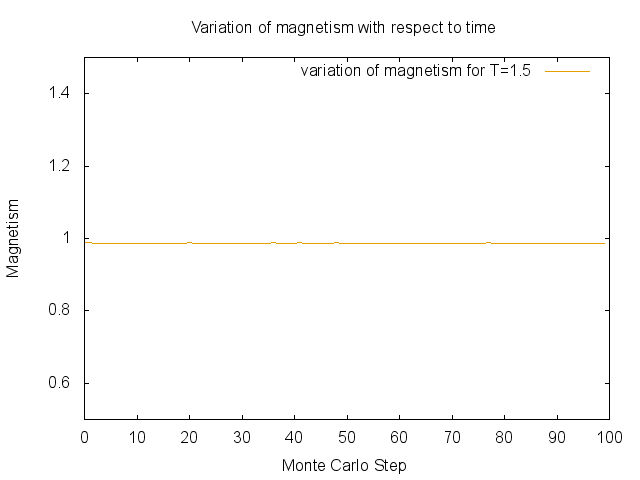
\includegraphics[scale=.8]{15.png}
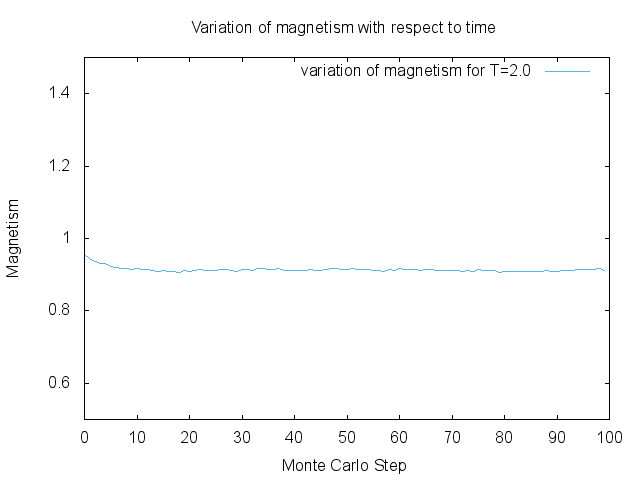
\includegraphics[scale=.8]{20.png}
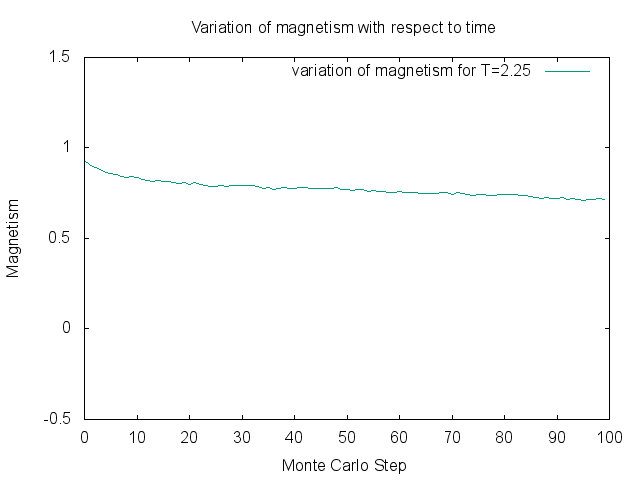
\includegraphics[scale=.8]{225.png}
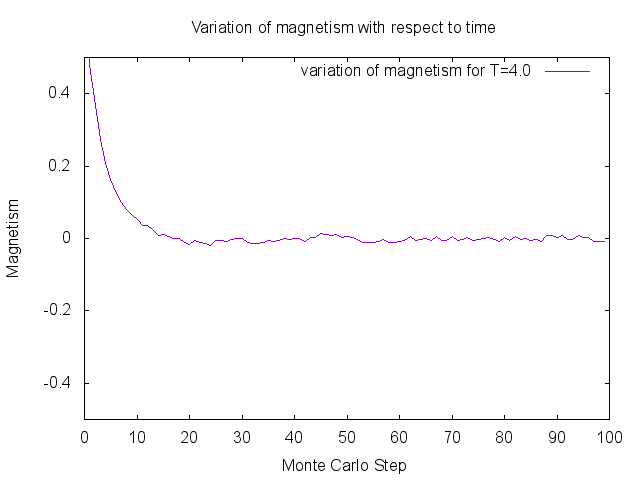
\includegraphics[scale=.8]{40.png}
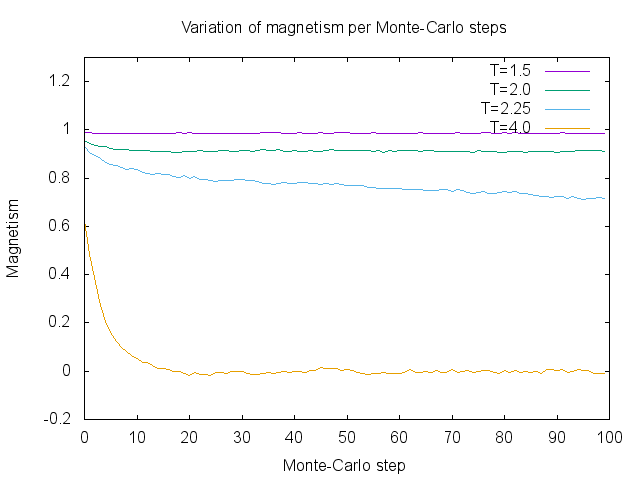
\includegraphics[scale=.8]{0.png}
\end{center}

نتایج برای 1000 گام به صورت زیر است.

\begin{center}
 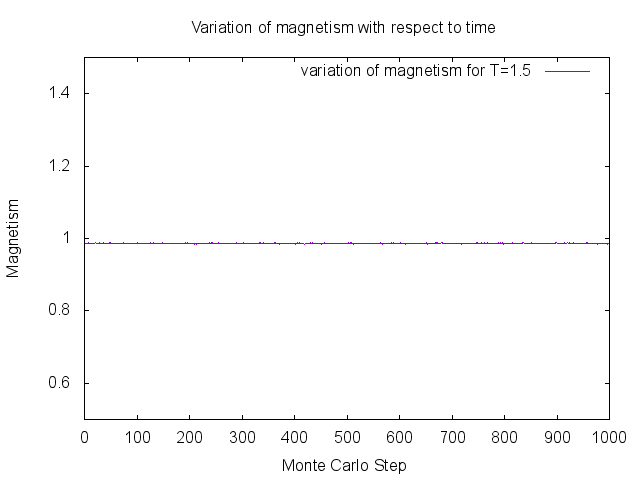
\includegraphics[scale=.8]{15A.png}
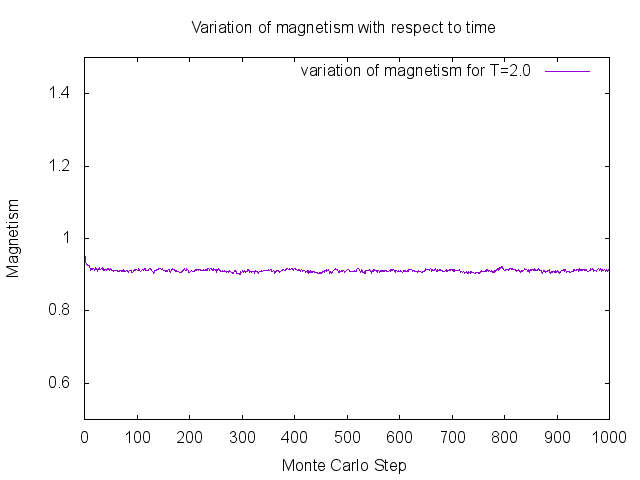
\includegraphics[scale=.8]{20A.png}
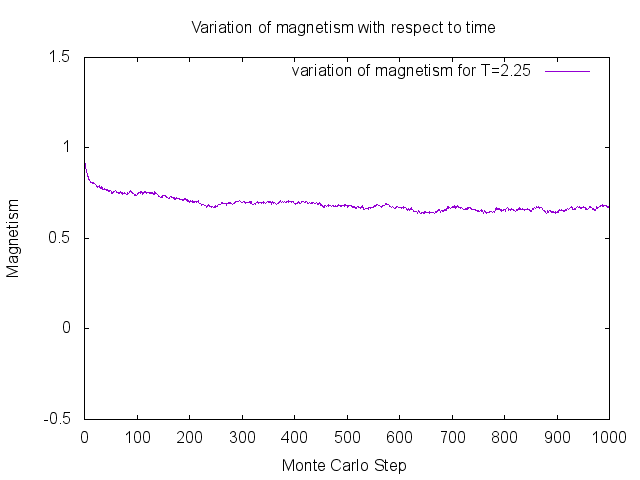
\includegraphics[scale=.8]{225A.png}
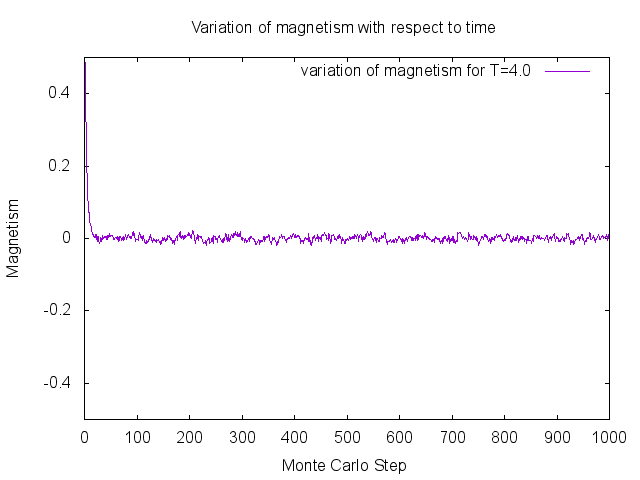
\includegraphics[scale=.8]{40A.png}
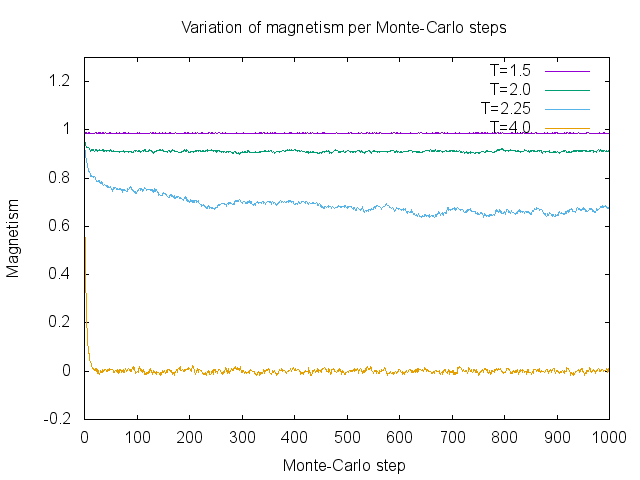
\includegraphics[scale=.8]{0A.png}
\end{center}
\section{میدان مخالف صفر}
این نتایج برای میدان مغناطیسی صفر و شرایط اولیه‌ای که همه‌ی
اسپین ها بالا هستند بود.
حال ما میدان مغناطیسی را غیر صفر فرض می‌کنیم
و در این بررسی میدان را  0.1، 0.2، 0.3، 0.4، 0.5، 0.6 و 0.7
قرار دادیم که منجر به نتایج زیر می‌شود.

\begin{figure}
\begin{center}
 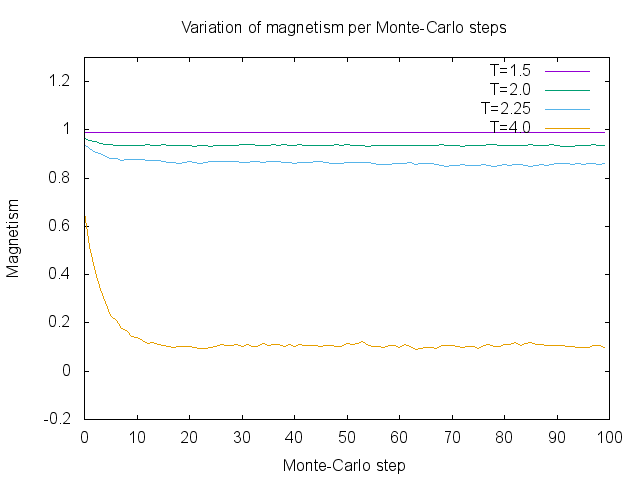
\includegraphics[scale=.8]{H0-1.png}\caption{میدان 0.1}
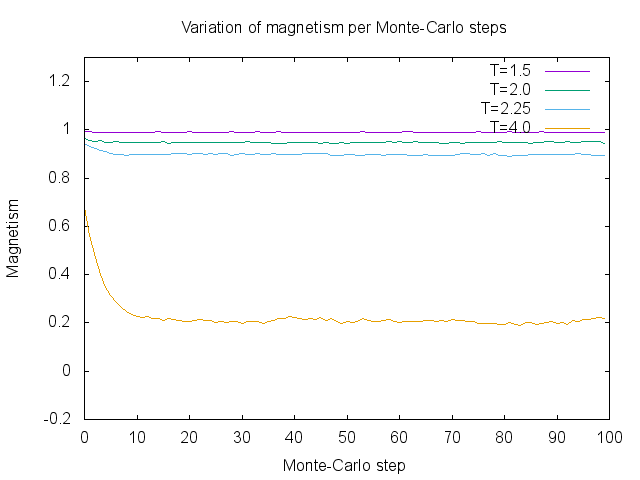
\includegraphics[scale=.8]{H0-2.png}\caption{میدان 0.2}
\end{center}
\end{figure}
\begin{figure}
\begin{center}
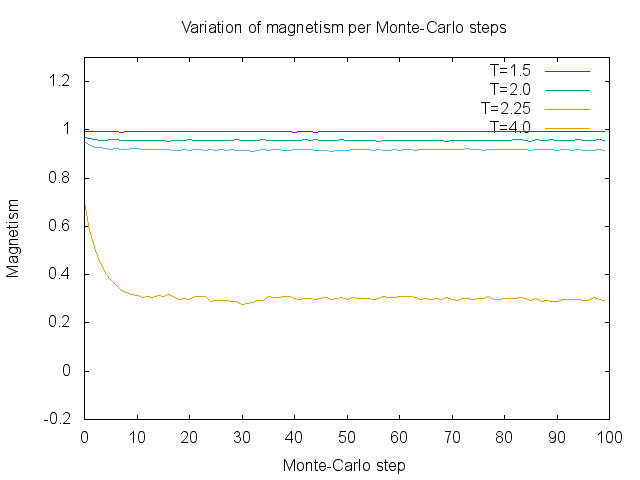
\includegraphics[scale=.8]{H-3.png}\caption{میدان 0.3}
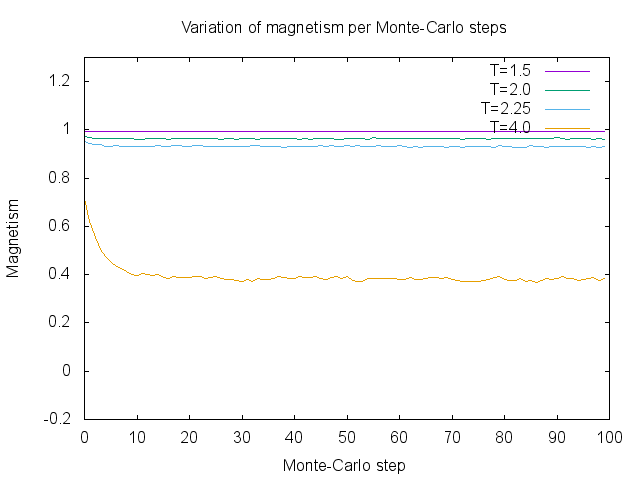
\includegraphics[scale=.8]{H-4.png}\caption{میدان 0.4}
\end{center}
\end{figure}
\begin{figure}
\begin{center}
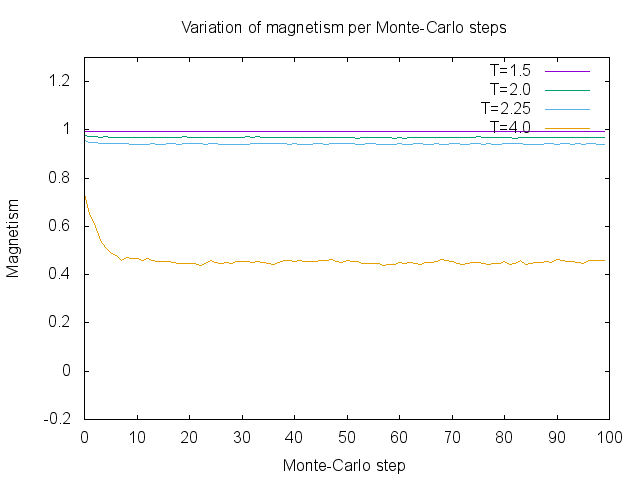
\includegraphics[scale=.8]{H-5.png}\caption{میدان 0.5}
 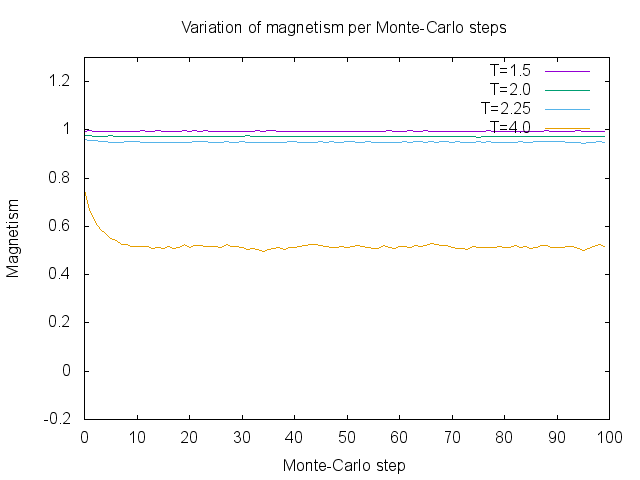
\includegraphics[scale=.8]{H-6.png}\caption{میدان 0.6}
 \end{center}
\end{figure}
\begin{figure}
\begin{center}
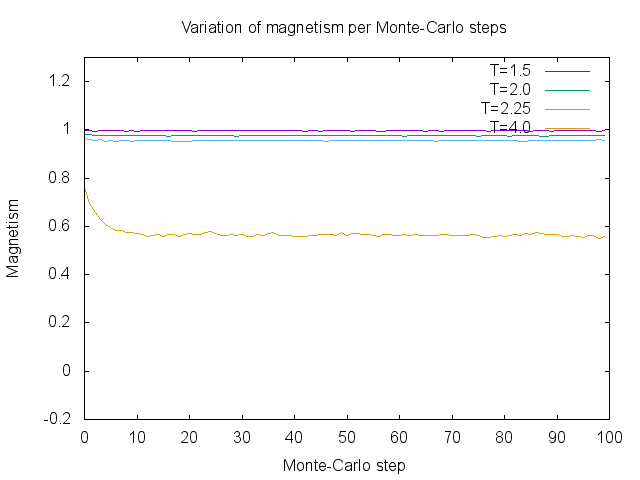
\includegraphics[scale=.8]{H-7.png}\caption{میدان 0.7}
\end{center}
\end{figure}


با توجه به نمودار‌های بالا همان‌طور که مشخص است در حالت تعادل سیستم در دمای 4
مغناطش غیر صفر دارد.
هرچه میدان افزایش پیدا کند، در دمای 4 درجه حالت تعادلی مغناطش بالاتری خواهیم داشت.
این موضوع باعث می‌شود که ما برای دماهای بالاتری حالت تعادلی با مغناطش صفز خواهیم داشت.
میدان به عنوان یک عامل مقاومتی در سیستم ظاهر می‌شود
که باعث می‌شود در دما‌های بالاتری دما بتواند بر این مولفه‌ی مقاومتی غلبه کند.

\section{نتایج پارامترها‌ی فیزیكی}
حال که دیدیم سیستم با توجه به دمایی که در آن است، در چه گامی به
تعادل می‌رسد، یک حلقه در کد قرار می‌دهیم و به سیستم اجازه
می‌دهیم به تعادل برسد.
بعد از به تعادل، یک حلقه‌ی دیگر در برنامه قرار می‌دهیم
و به اندازه‌ی 100 قدم مونته کارلو اجازه‌ی اجرا می دهیم.
در هر کدام از این گام‌ها مقادیر فیزیكی مورد نظر را محاسبه می‌کنیم.
بعد از تمام شدن این حلقه از کمیت‌های فیزیکی که در هر گام به دست آمد متوسط گیری می‌کنیم.
این متوسط گیری شامل تقسیم کردن تیجه به تعداد قدم‌های مونته کارلو است.
نتایج به شکل زیر است:
\begin{center}
 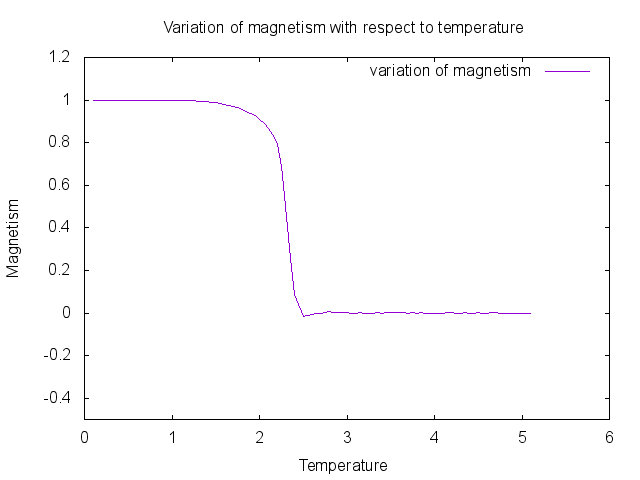
\includegraphics[scale=.8]{MPT.png}
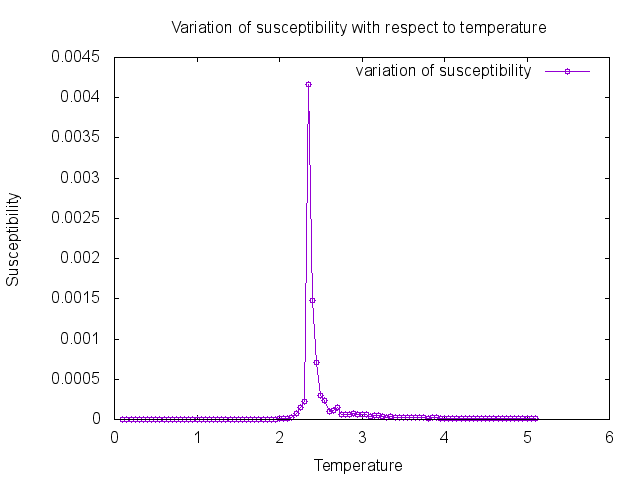
\includegraphics[scale=.8]{SUS.png}
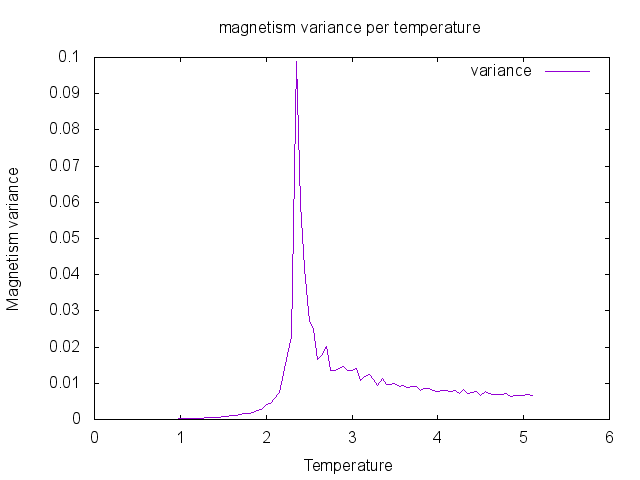
\includegraphics[scale=.8]{VARM.png}
\end{center}

در این نتایج متوجه می‌شویم که در یک دمای خاص که بین
2.25 و 2.5 است یک تغییر در سیستم رخ می‌دهد.
مغناطش در این دما به صفر می‌رسد که این موضوع گذار متبه اول سیستم را نشان می‌دهد.
در این گذار ما یک شکست تقارن برای سیستم دارسم که مغناطش از یک مقدار خاص به صورت 
ناگهانی به صفر می‌رسد.
در نمودار پذیرفتاری نیز مشاهده می‌شود که یک پیک در دمای
بحرانی برای سیستم داریم.
پس در دمای بحرانی سیستم رفتار خاصی از خود نشان می‌دهد و نمی‌توان کمیت های 
فیزیكی را به‌خوبی بررسی کرد.
\subsection{دمای بحرانی}
در این بررسی برای پذیرفتاری سیستم ما تلاش کزردیم تا برای سیستم
دمای بحرانی را پیدا کنیم.
دمای بحرانی نقطه‌ای از نمودار پذیرفتاری بر حسب دما است که مقدار پذیرفتاری
ماکزیمم است.
پنوک قله‌ی این نمودار به ما دمای بحرانی
را میدهد.
در این بررسی مقداری که ما برای دمای بحرانی پیدا کردیم 2.4 بود.
در این دما و همسایگی آن به دنبال پیدا کردن نمای بحرانی هستیم.
این کار را با کد زیر در
\lr{gnuplot}
انجام می‌دهیم.
کد این کار به صورت زیر است و نتیجه نیز در شکل پایین آمده است.
\begin{lstlisting}
            magnTemp<<"set title\"Variation of magnetism with respect to temperature\"\n"
                   <<"set terminal png \n"
                   <<"set output \"FIT.png\"\n"
                   <<"set ylabel \"Magnetism\"\n"
                   <<"set xlabel\"Temperature\"\n"
                    << "set autoscale \n"
                    << "beta=0.12 \n"
                    << "g(x)=x>0?(x<2.4?a*(2.4-x)**beta:0):0 \n"
                    << "fit g(x) '-' using 1:2 via a,beta \n"
                    << "set term x11" << endl;	
\end{lstlisting}
\begin{center}
 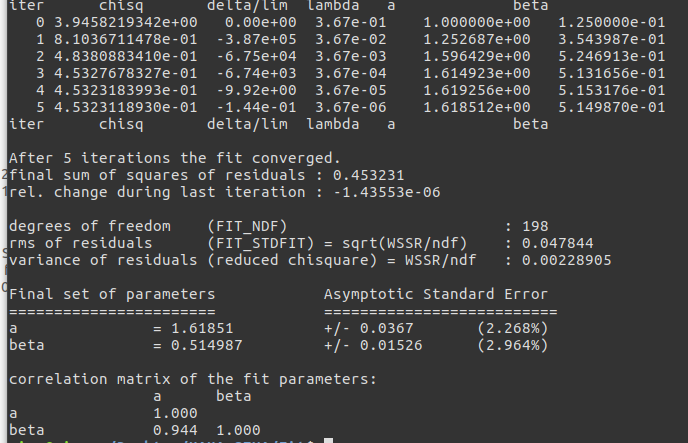
\includegraphics[scale=.3]{10.png}
\end{center}
همان طور که دیده می‌شود این نمای بحرانی 0.514987
به دست می‌اید.
\section{ثبت تغییرات سیستم و ایجاد فیلم }
در یک قسمت از این بررسی ما به دنبال ایجاد یک روش برای مشاهده بصری سیستم بودیم.
به این منظور ما به دنبال ثبت و ضبظ حالت سیستم در دما‌های مختلف بودیم.
در این کار ما با تغییر جزئی دمای سیستم، به سیستم اجازه دادیم تا به تعادل برسد
و در نهایت اندازه‌ی اسپین ها را ثبت کردیم.
در این حالت به تعداد زیادی فایل متنی ایجاد کردیم که هرکدام یک موقعیت از
سیستم را در دمای خاص توصیف می‌کند.
حال باید این فایل‌های متنی را به صورت یک عکس درست کنیم.
فایل ایجاد شده در اینجا یک فایل متنی است که یک ماتریس
$256\times256$
است که درایه‌های آن صفر و یک هستند.
تولید عکس از یک فایل متنی را میتوان در نرم‌افزار متلب یا اکتاو با یک دستور
\lr{imagesc(A)}
انجام داد، که
\lr{A}
در اینجا همان فایل متنی بارگذاری شده است.
در نهایت می‌توان همه عکس‌ها را به هم وصل کرد و یک فایل ویدیویی
تولید کرد.
به دلیل زیاد بودن این فایل‌های متنی ما از
یک دستور دیگر در نرم‌افزار
\lr{gnuplot}
استفاده کردیم و همه فایل های متنی را با هم به عکس تبدبل کردیم.
و در نهایت در لینوکس با دستور
\lr{convert}
این عکس‌ها را به فیلم تبدیل کردیم.
کدی که برای تبدیل فایل متنی به عکس نوشتیم به شکل زیر است:
\begin{lstlisting}
 #!/usr/bin/gnuplot
set terminal png
set cbrange [0:1]
set key left
set palette defined (0 "red", 0.4999 "red", 0.5 "blue", 1 "blue")
set cbtics ("↓" 0.25, "↑" 0.75)
do for [T=25:500:10] {
do for [s=1:199:5] {
temp=T/100.
set output sprintf('pic/snapshot-%.2f-%d.png',temp,s)
print sprintf('snapshot/snapshot-%.2f-%d.txt',temp,s)
plot sprintf('snapshot/snapshot%.2f-%d.txt',temp,s) matrix with image title sprintf('T=%.2f step=%d',temp,s)
}
}
\end{lstlisting}

\section{همبستگی سیستم}
در این قسمت ما به دنبال این هستیم که که همبستگی سیستم را محاسبه کنیم.
همبستگی سیستم به دما بستگی دارد، پس در دما‌های متفاوت باید
نتایج متفاوتی برای همبستگی داشته باشیم.
رابطه‌ی همبستگی به شکل زیر است:
$$
f(i)=<s_0s_i>
$$
$$
f(i)\propto e^{-r_i/\xi}
$$
$$
\xi\sim\frac{1}{|T-T_c|^\nu}
$$
در رابطه‌ی بالا
$\xi$
ظول همبستگی را برای ما مشخص می‌کند.
این پارامتر را می توان از روی نمودار همبستگی بر حسب همسایه‌ها
به‌دست آورد.

محاسبات ما برای همبستگی به این صورت است که اسپین با 
اندیس 128 را انتخاب کردیم و همبستگی آن را با همه‌ی
همسایه‌هایش محاسبه کردیم.
این همبستگی را در هر قدم مونته کارلو محاسبه کردیم و در نهایت یک میانگین‌گیری
روی کل این قدم‌ها انجام دادیم.
لازم به ذکر است که سیستم ما در این جا
$256\times256$
است و ما اسپین 128 را برای برسی انتخاب کردیم.
از آن‌جایی که این همبستگی به دما بستگی دارد
 پس می‌توان این کار را برای دماهای متفاوت انجام داد.
 ما این کار را برای دماهای 1.5، 2، 2.25، و 3 انجام دادیم.
 نتیجه این بررسی به شکل زیر است:

\begin{center}
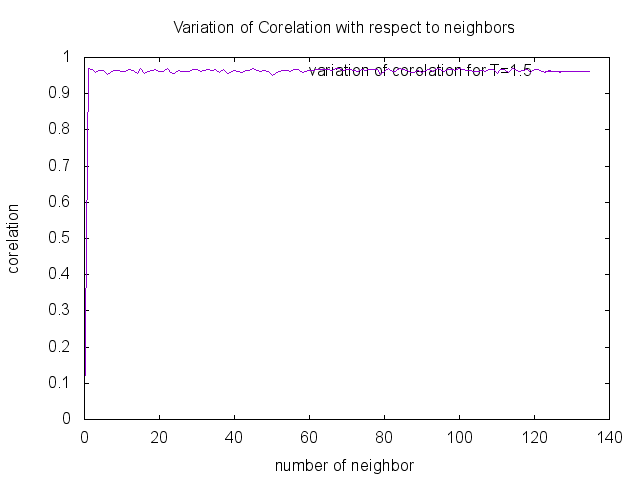
\includegraphics[scale=.8]{C1.png}
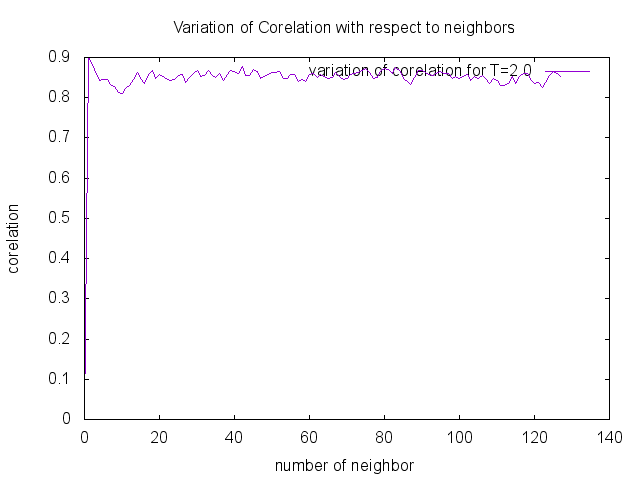
\includegraphics[scale=.8]{C2.png}
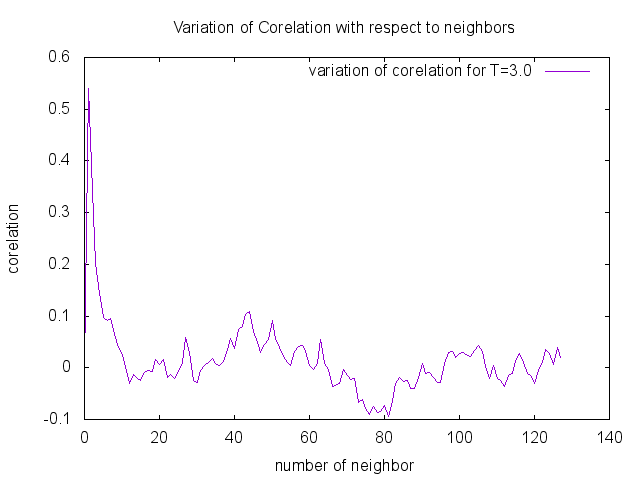
\includegraphics[scale=.8]{C3.png}
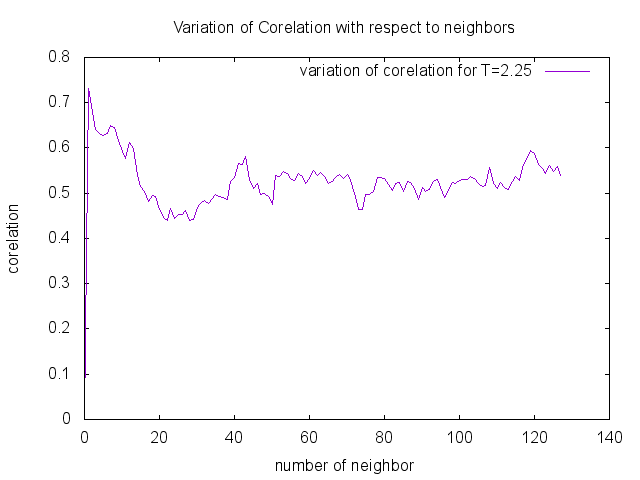
\includegraphics[scale=.8]{C5.png}
\end{center}

همان‌گونه که از نمودار‌های بالا مشخص است
در دما‌های پایین همبستگی زیاد است و تا همسایه‌های خیلی
دور هم مقدار زیادی دارد.
با افزایش دما همبستگی برای همسایه‌های 
دورتر کاهش پیدا می‌کند. برای مثال در دمای 3 این مقدار برای
همسایه‌های خیلی دور به صفز می‌رسد.
این موضوع را می‌توان به صورت حوضه های مغناطیسی تغبیر کرد.
در دما‌های کم حوضه‌های مغناطیسی بزرگ است، به صورتی که در دمای یک همه‌ی اسپین‌ها
در یک جهت هستند و مغناطش سیستم بزرگ است.
با افزایش دما همبستگی کاهش پیدا می‌کند
و متناظر با این کاهش همبستگی می‌توان گفت که حوضه‌های مغناطیسی
کوچک می‌شوند.
در دماهای بالا این مقدار به صفر می‌رسد
چرا که همه‌ی اسپین ها به صورت تصادفی جهت‌گیری می کنند.
در دمای بحرانی مقدار همبستگی باید بی‌نهایت شود.
ولی چون سیستم در حد تزمودینامیکی نیست این اتفاق نمی‌افتد.

 در ادامه ما همبستگی را در دمای بحرانی حساب کردیم.
 همبستگی در دمای 2.4 به شکل زیر است:
\begin{center}
 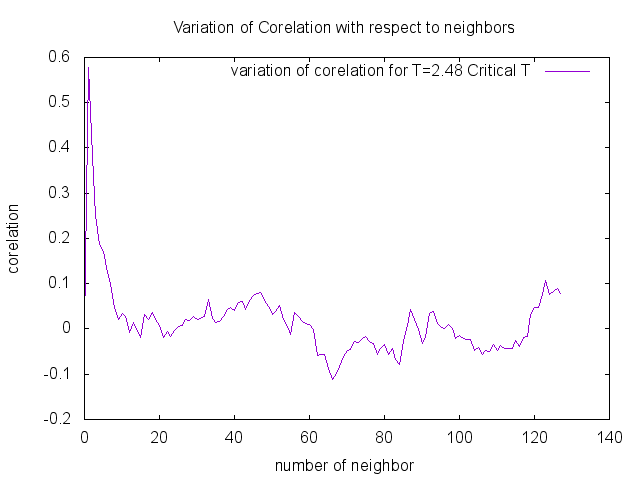
\includegraphics[scale=1]{C6.png}
\end{center}

\end{document}          




